\documentclass[titlepage]{article}
\usepackage[14pt]{extsizes} 
\usepackage[T2A]{fontenc}
\usepackage[utf8]{inputenc}
\usepackage[english,russian]{babel}
%\usepackage{pscyr}
\usepackage{hyperref}
\usepackage{setspace}
\usepackage{amsmath,amssymb,amsfonts,amsthm,secdot}
\usepackage[left=30mm, top=20mm, right=30mm, bottom=20mm, nohead, footskip=15mm]{geometry} 
\usepackage[pdftex]{graphicx}
\usepackage[indentfirst]{titlesec}
\usepackage[usenames]{color}
\usepackage{colortbl}
\usepackage{listings}
\usepackage{secdot}
\usepackage{graphicx}

\def\l{\left}
\def\r{\right}
\def\le{\leqslant}
\def\ge{\geqslant}

\begin{document} 

\newtheorem{theorem}{Теорема}
\newtheorem{lemma}{Лемма}
\newtheorem{definition}{Определение}
\renewcommand{\proofname}{Доказательство}

\newpage
\begin{center}
\Large \textbf{Московский Государственный Университет}\\
\hfill \break
\Large \textbf{имени М.В.Ломоносова}\\
\hfill \break
\hfill \break
\hfill \break
\hfill \break
Механико-математический факультет\\
Кафедра теоретической информатики\\
\hfill \break
\hfill \break
\hfill \break
\LARGE Методы трассировки лучей \\
\hfill \break
\large Д.А. Михайлин \\
\hfill \break
\today \\

\end{center}

\newpage
\section{Основные определения.}
Основная задача всех алгоритмов рендеринга - это создать изображение виртуальной сцены. Алгоритмы трассировки лучей решают эту проблему следующим образом: они эмулируют физическое поведение света. Рассчитывают его отражение, поглощение различными элементами сцены. Результатом работы алгоритма является изображение, полученное виртуальной камерой.
\subparagraph{} Так как, все эти алгоритмы опираются на физическое поведение света, то необходимо дать определение некоторым физическим величичнам, которые используются для расчета поведения лучей.
\subparagraph{} Основной такой физической величиной является \textbf{поток излучения}.\\
\textbf{Поток излучения}(Flux) характеризует мощность, переносимую оптическим излучением через какую-либо поверхность. Равен отношению энергии, переносимой излучением через поверхность, ко времени переноса.
\begin{gather} 
	\Phi = \frac{dQ}{dt}
\end{gather}
\begin{center}
	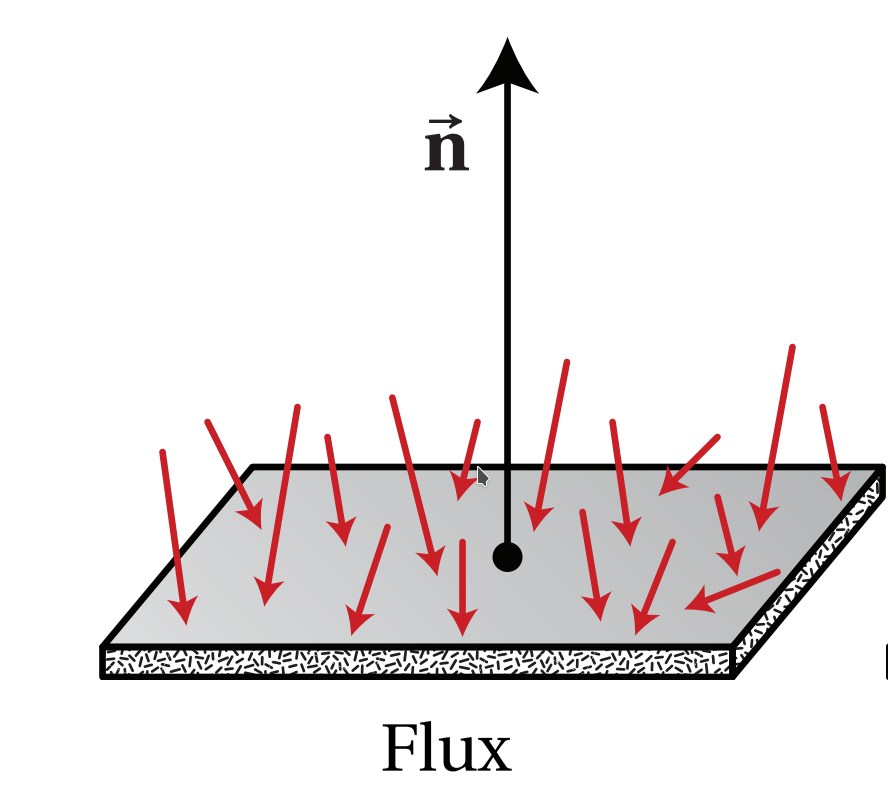
\includegraphics[scale=0.5]{Flux.png}
\end{center}
\subparagraph{} \textbf{Интенсивность излучения}(Irradiance) - это поток излучения, получаемый или излучаемый поверхностью на единице площади. Поток рассматривается через весь телесный угол $\Omega$. Обозначается буквой E.
\begin{gather}
	E = \frac{d\Phi(x)}{dS(x)}; \\E =  \bigg[\frac{W}{m^{-2}}\bigg]
\end{gather}
\begin{center}
	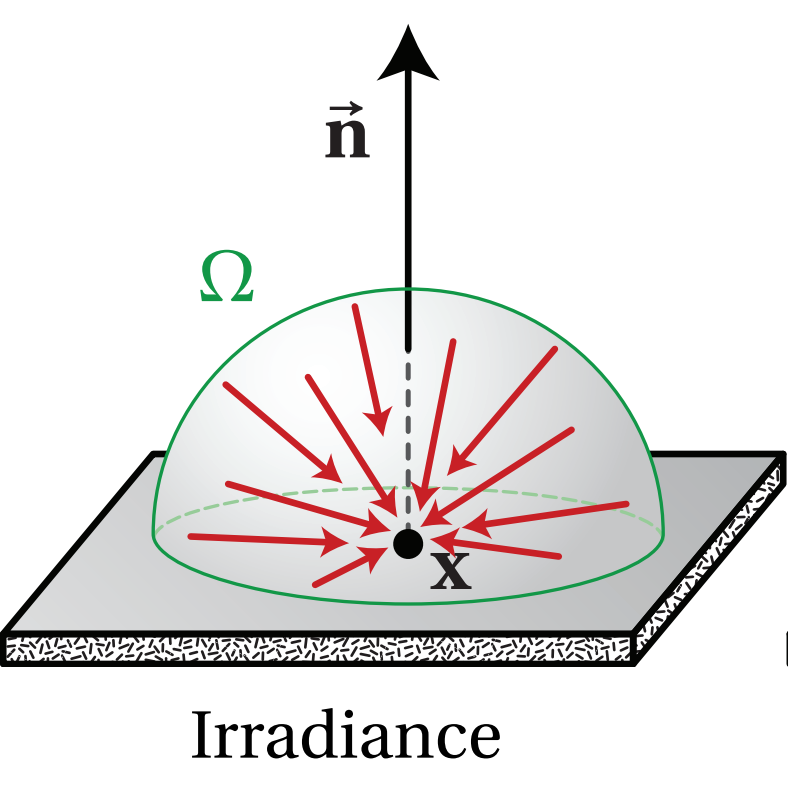
\includegraphics[scale=0.5]{Irradiance.png}
\end{center}
\subparagraph{} \textbf{Светимость}(Radiance) -  отношение потока излучения, испускаемого с бесконечно малой площадки источника и распространяющегося в бесконечно малом телесном угле, к площади проекции этой площадки на плоскость, перпендикулярную направлению распространения, и величине телесного угла. Обозначается $L$.
\begin{gather}
	L(x, \omega) = \frac{d^2\Phi(x)}{d\omega(x)dA^{\perp}(x)}\\
	L(x, \omega) = \frac{d^2\Phi(x)}{d\omega^{\perp}(x)dA(x)} \\
	L = \bigg[\frac{W}{Sr*m^2}\bigg]
\end{gather}
\begin{center}
	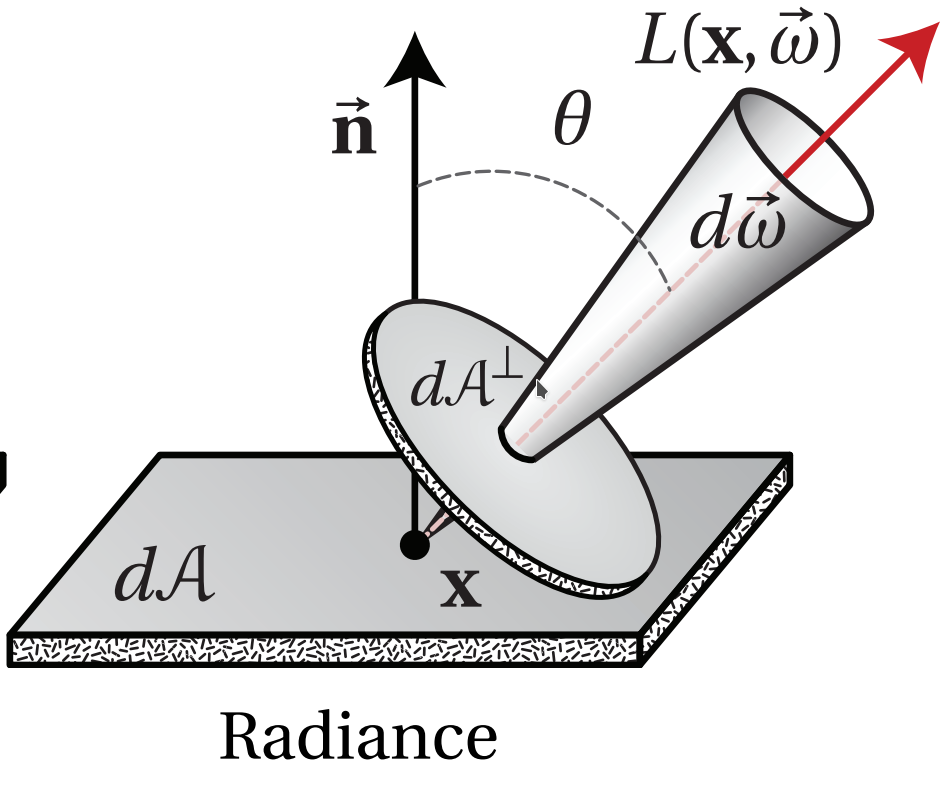
\includegraphics[scale=0.5]{Radiance.png}
\end{center}
%Требуется приближенно вычислить интеграл: 
%\begin{gather}
%	\int_{0}^{+\infty}(x + \frac{1}{x})\frac{(sin{3x})^2}{\ln(1 + x)}e^{-x^2}dx
%\end{gather}
%с заданной точностью $\varepsilon = 10^{-2}$.

\section{Связь между этими величинами}
Мы можем переписать $dA^{\perp} = (n, \omega)dA$ . Так же, можно записать $d\omega^{\perp} = (n, \omega)d\omega$. Следовательно верны следующие формулы:
\begin{gather}
	L(x, \omega) = \frac{d^2\Phi(x)}{d\omega(x)dA^{\perp}(x)} = \frac{d^2\Phi(x)}{(n,\omega)d\omega(x)dA(x)} = \frac{d^2\Phi(x)}{d\omega^{\perp}(x)dA(x)}
\end{gather}
\subparagraph{} Выразим теперь поток излучения через светимость. Проинтегрируем сначала по полусфере, получив интенсивность излучения, а потом проинтегрируем по площади, для которой и считаем поток.
\begin{gather}
	L(x,\omega)d\omega(x)dA^{\perp}(x) = d^2\Phi(x)\\
	\Phi(x) = \int_A \int_{\Omega} L(x, \omega)d\omega(x)dA^{\perp}(x) = \\ \int_A \int_{\Omega} L(x, \omega)(\omega, n)d\omega(x)dA(x) = \\ \int_A \int_{\Omega} L(x, \omega)d\omega^{\perp}(x)dA(x)
\end{gather}
\subparagraph{} Выразим теперь интенсивность излучения через светимость. 
\begin{gather}
	E(x) = \int_{\Omega}L(x,\omega)(\omega, n)d\omega = \int_{\Omega}L(x, \omega)d\omega^{\perp}
\end{gather}
\section{BRDF}
	Введем новые обозначения для светимости. \\
	$L(x\rightarrow\omega)$ - функция, которая описывает поток, исходящий из точки x в направлении $\omega$. \\
	$L(x\leftarrow\omega)$ - функция, которая описывает поток, попадающий в точку x по направлению $\omega$. 
\subparagraph{} \textbf{Bidirectional reflectance distribution function}(BRDF) - функция, которая описывает каким образом свет отражается от непрозрачной поверхности. Она показывает насколько "ярко"  выглядит поверхность с направления $\omega$.
\begin{gather}
	f_r(x, \omega_1\rightarrow\omega) = \frac{dL(x\rightarrow\omega)}{dE(x\leftarrow\omega_1)} = \frac{dL(x\rightarrow\omega)}{L(x\leftarrow\omega_1)(n,\omega_1)d\omega_1}
\end{gather}
\begin{center}
	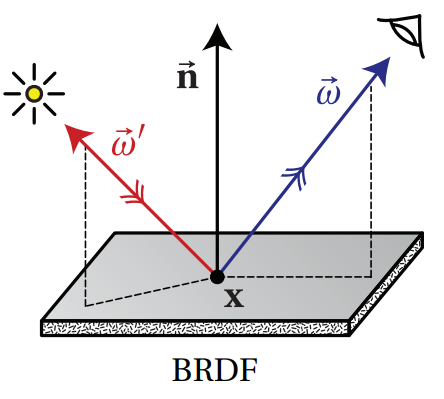
\includegraphics[scale=0.5]{BRDF.png}
\end{center}
\section{Основное уравнение рендеринга}
	\textbf{Основное уравнение рендеринга} описывает исходящее излучение $L(x\rightarrow\omega)$ из произвольной точки сцены, как сумму испускаемого излучения и отраженного излучения. 
\begin{gather}
	L_o(x\rightarrow\omega) = L_e(x\rightarrow\omega) + L_r(x\rightarrow\omega)
\end{gather} 
\subparagraph{} Используя выражение для BRDF перепишем уравнение рендеренга:
\begin{gather}
	f_r(x, \omega_1\rightarrow\omega) = \frac{dL(x\rightarrow\omega)}{L(x\leftarrow\omega_1)(n,\omega_1)d\omega_1} \\
	dL(x\rightarrow\omega) = f_r(x, \omega_1\rightarrow\omega)L(x\leftarrow\omega_1)(n,\omega_1)d\omega_1
	\\
	L(x\rightarrow\omega) = \int_{\Omega}f_r(x,w \rightarrow w')L(x\leftarrow\omega')(n,\omega')d\omega'
	\\L(x\rightarrow\omega) = L_e(x\rightarrow\omega) + \int_{\Omega}f_r(x,w \rightarrow w')L(x\leftarrow\omega')(n,\omega')d\omega'
\end{gather}
\section{Метод Монте-Карло}
Основная проблема в решении уравнения рендеринга состоит в том, что необходимо проинтегрировать функцию 
$L(x\rightarrow\omega')$, которая неизвестна. Таким образом сложно сделать какие-либо предположения о  ее поведении. Необходимо слишком много лучей, чтобы узнать что-либо о поведении данной функции. Поэтому приходиться использовать вероятностные методы подсчета этого интеграла.\\
Рассмотрим интеграл вида $I = \int_a^b\phi(x)dx$. Ведем случайную величину $\xi$ , которая равномерно распределена. Следовательно интеграл будет выражаться через матожидание след. образом:
\begin{gather}
	E[\phi(\xi)] = \int_a^b\phi(x)f(x)dx = \frac{1}{b - a} \int_a^b\phi(x)dx \\
	\int_a^b\phi(x)dx = (b - a)E[\phi(x)]
\end{gather}
Заменим математическое ожидание его оценкой - выборочным средним.
\begin{gather}
	I^{*} = (b - a)\frac{\sum_{i = 1}^N\phi(x_i)}{N}
\end{gather}
Рассмотрим теперь общий случай. \\
	Для вычисления интеграла введем функцию f(x) - плотность распределения случайной величины $\xi$.
\begin{gather}
	\int_a^bf(x)dx = 1
\end{gather}
	Представим интеграл в виде:
\begin{gather}
	\int_a^b\frac{\phi(x)f(x)}{f(x)}dx = E\bigg[\frac{\phi(x)}{f(x)}\bigg]
\end{gather}
Для оценки интеграла будем использовать выборочное среднее:
\begin{gather}
	I_2^{*} = \frac{1}{N}\sum_{i = 1}^N\frac{\phi(x_i)}{f(x_i)} 
\end{gather}
Рассмотрим точность данного алгоритма на различных распределениях.
\section{Результаты работы рендера}
\begin{center}
	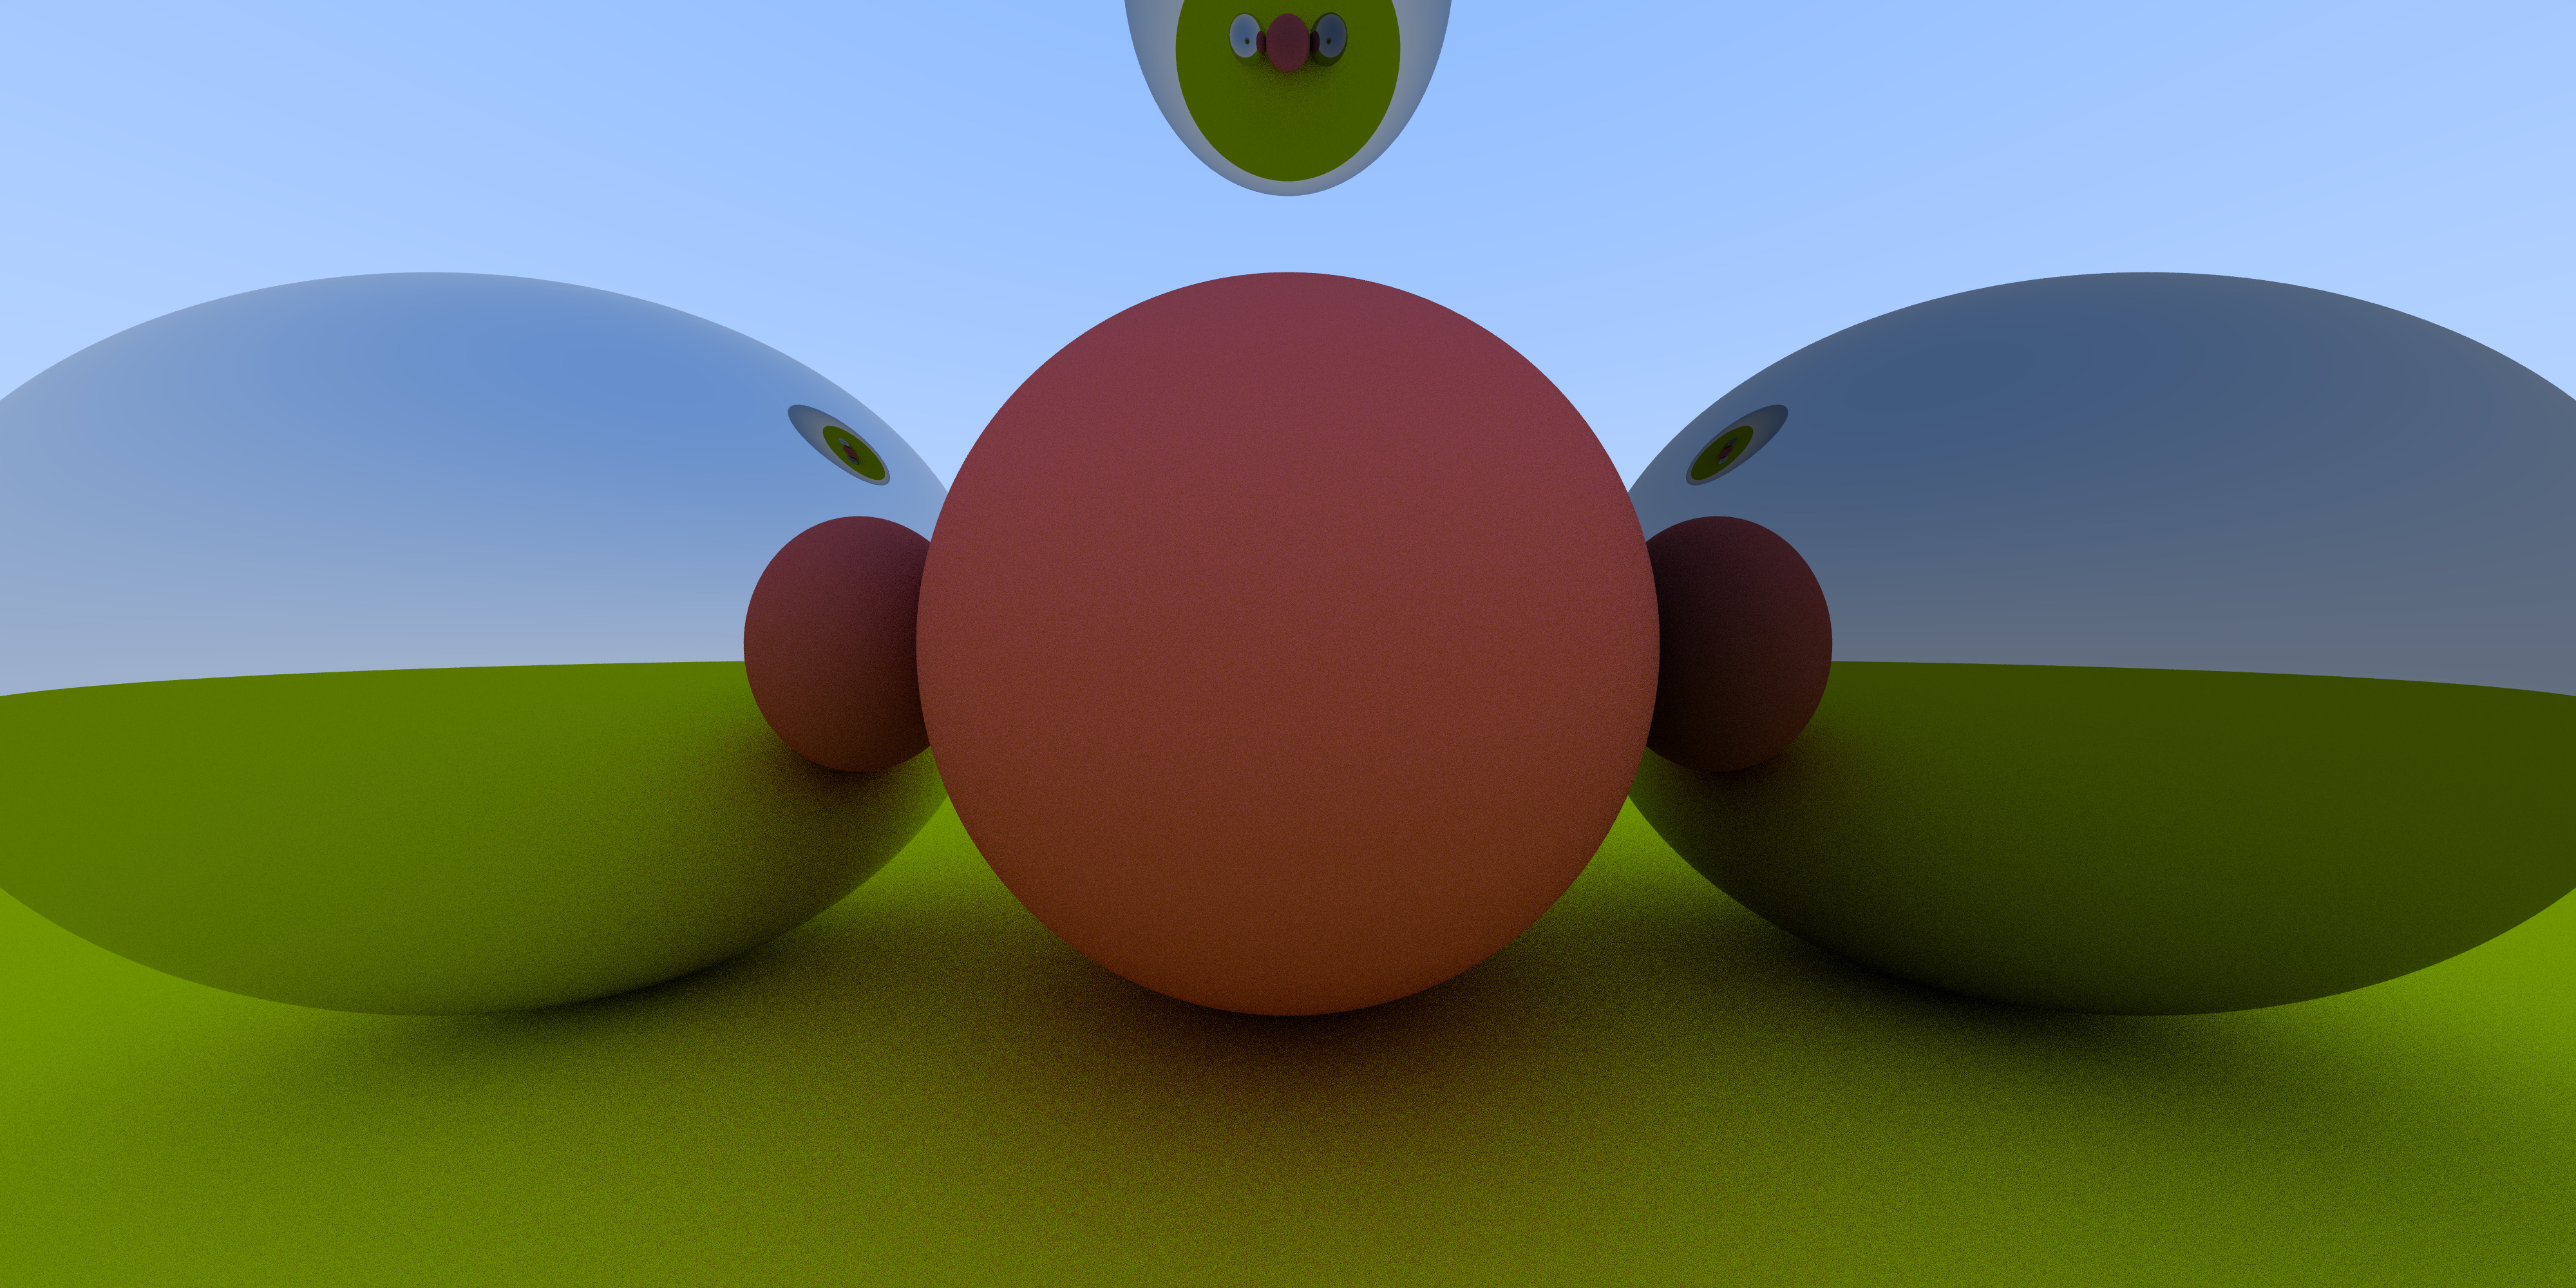
\includegraphics[scale=0.1]{fiveSpheres.jpg}
	\\Два ламбертиана.
	\\
\end{center}
\begin{center}
	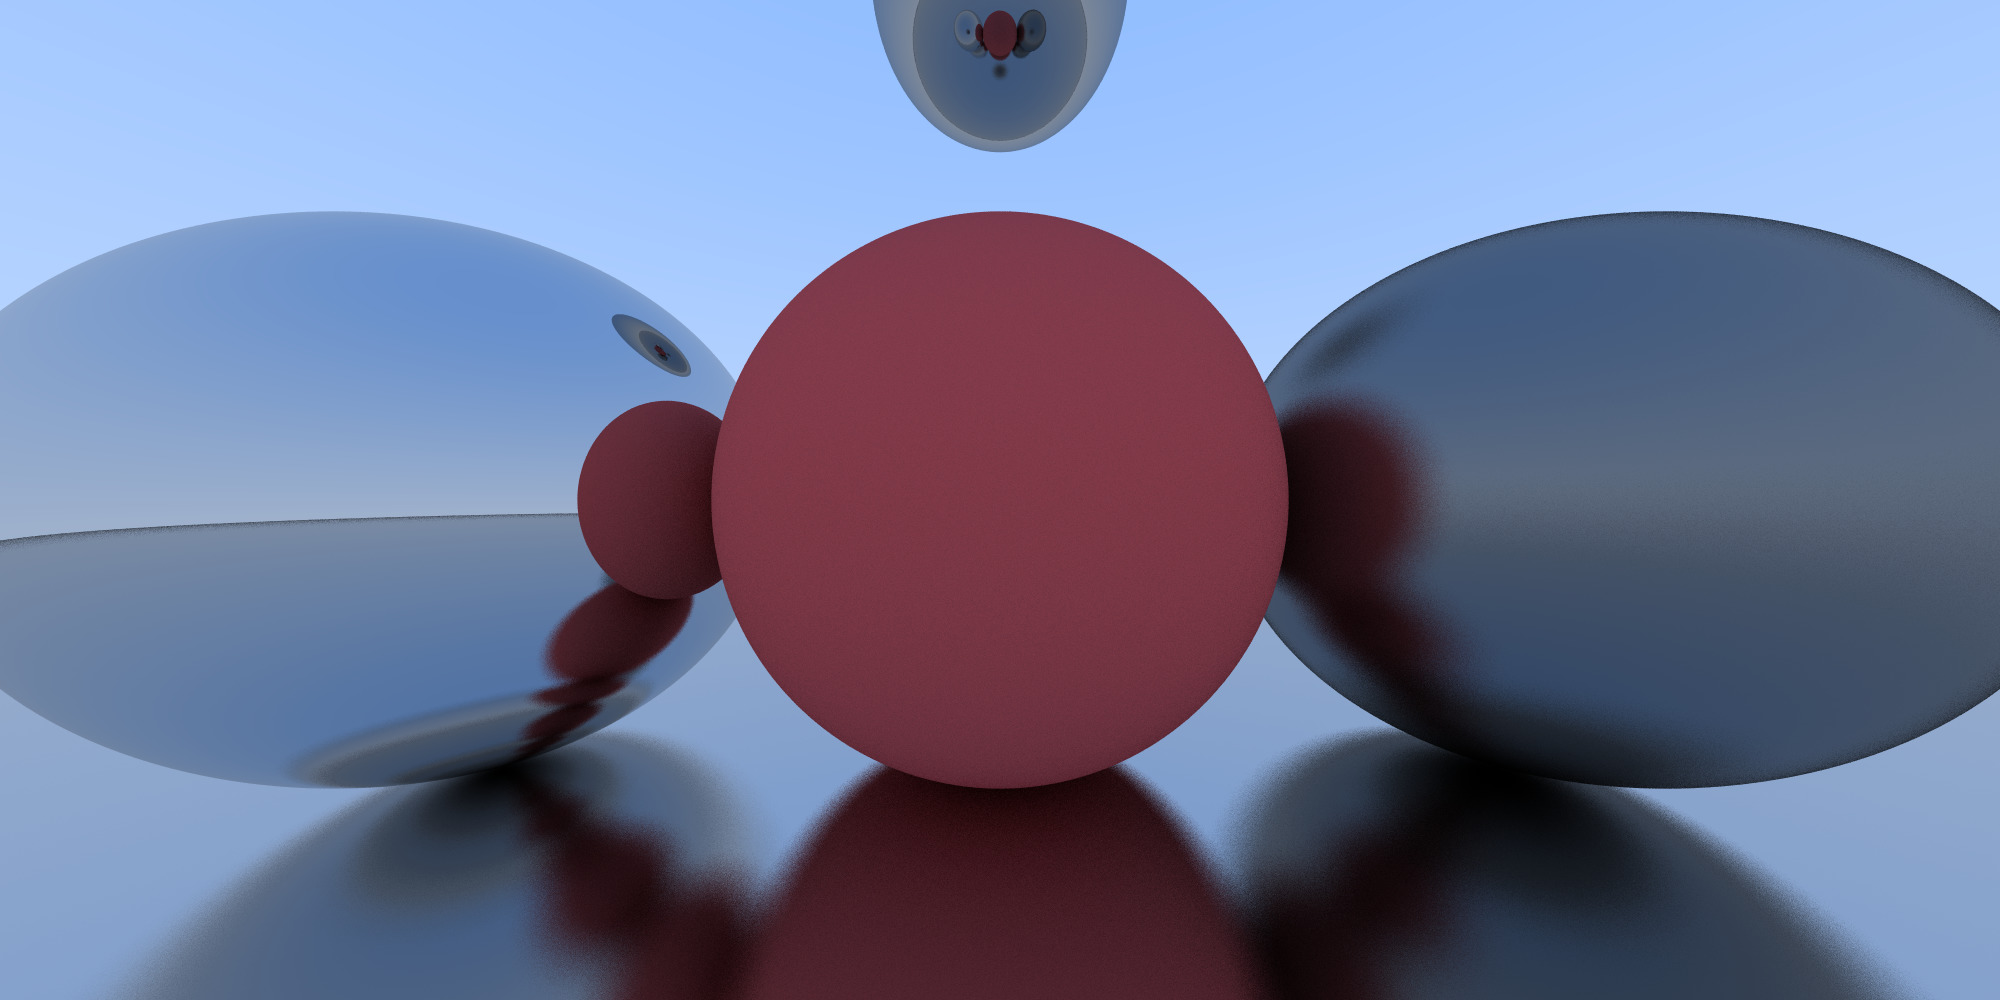
\includegraphics[scale=0.2]{fuzemetal.jpg}
	\\Не идеальное зеркало и ламбертиан.
\end{center}
\begin{center}
	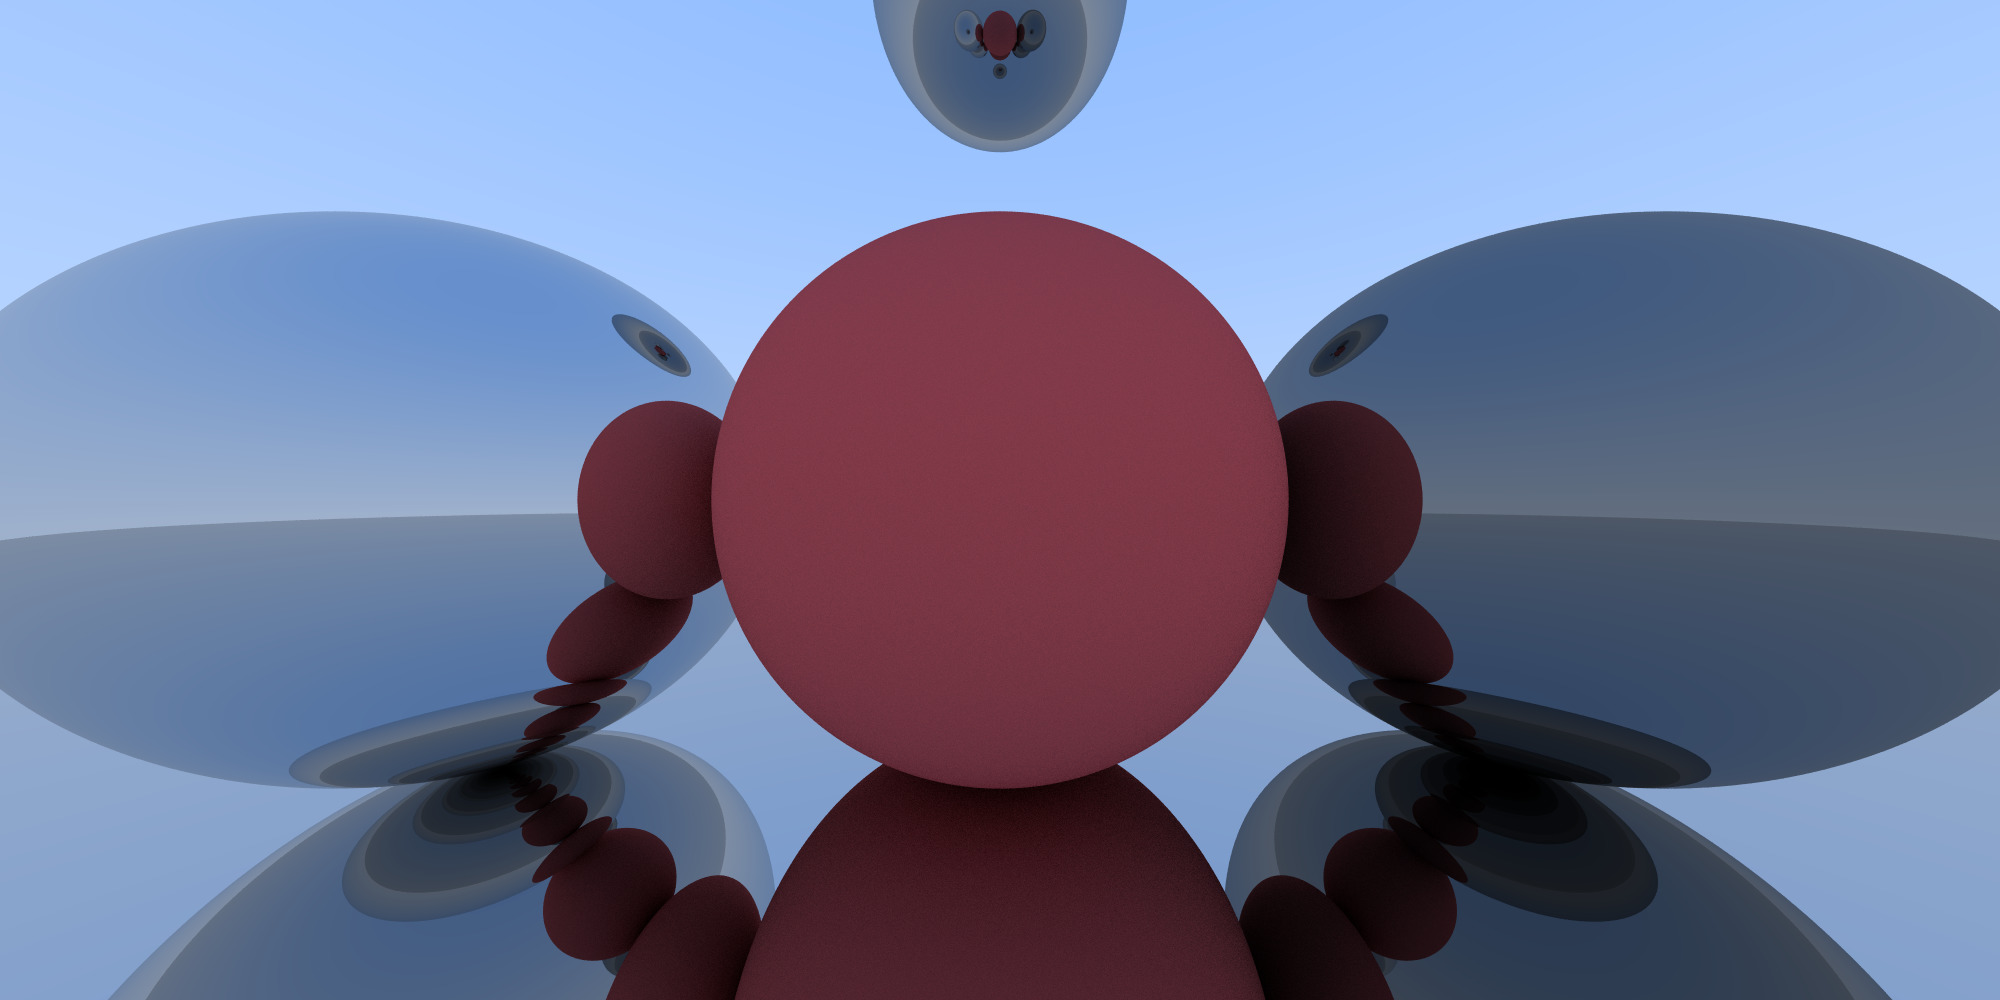
\includegraphics[scale=0.2]{metal.jpg}
	\\Идеальное зеркало и ламбертиан.
\end{center}
\begin{center}
	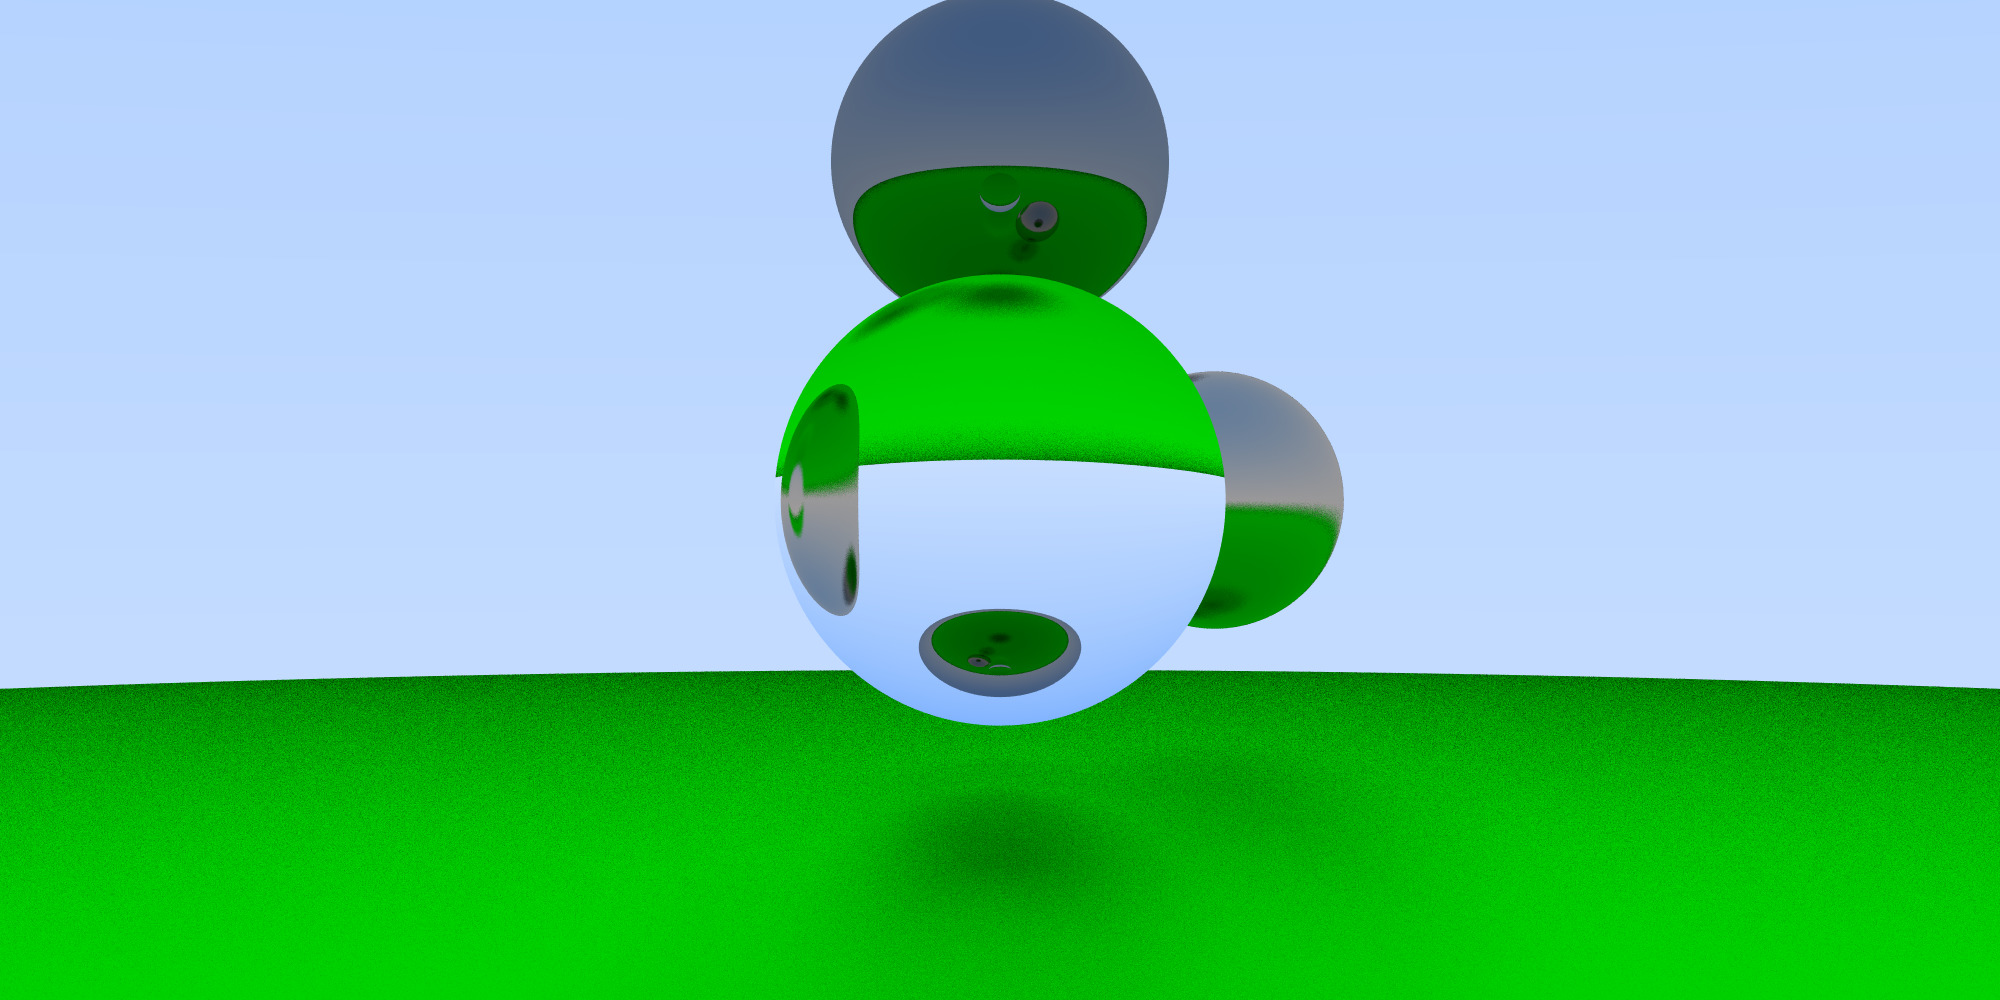
\includegraphics[scale=0.2]{wtf.jpg}
	\\Cтеклянная сфера.
\end{center}
\newpage
\textbf{Список Литературы}
\\
1) "Efficient Monte Carlo Methods for light transporn in scattering media" A dissertation submitted in partial satisfaction of the
requirements for the degree
Doctor of Philosophy
in
Computer Science
by
Wojciech Jarosz
\\
2)Philip Dutré, Philippe Bekaert, and Kavita Bala. Advanced Global Illumination. AK Peters, Ltd.,
second edition, 2006. 149, 178\\
3)Liu, B. Y. H.; Jordan, R. C. (1960). "The interrelationship and characteristic distribution of direct, diffuse and total solar radiation".
\end{document}